\section{度量的比较}
\label{sec:dep-comparison}

四类度量都从同一个问题出发：$P_{(X,Y)}$与$P_X\otimes P_Y$相差多少。它们在条件、零值、变换与刻度上的差别，决定了各自适合回答什么。

\paragraph{性质对照}
表~\ref{tab:dep-properties}把前面各节的结论放在一起。“零值刻画独立”一栏都是在所列条件下成立的；HSIC一栏指高斯核或其他使乘积核成为特征核的选择，线性核单独列出作为对照。

\begin{BookInlineTable}
  \centering
  \small
  \begin{tabular}{@{}p{15mm}p{22mm}p{13mm}p{26mm}p{20mm}@{}}
    \toprule
    度量 & 适用条件 & 零值刻画独立 & 保持不变的变换 & 取值与参数\\
    \midrule
    互信息 & 任意可测空间 & 是 & 双向可测一一映射 & $[0,\infty]$，无参数\\
    距离相关 & 欧氏空间，一阶矩 & 是 & 平移、正交、整体缩放 & $[0,1]$，无参数\\
    HSIC（高斯核） & 欧氏空间，无矩条件 & 是 & 平移、正交 & 非负，依赖带宽\\
    HSIC（线性核） & 实值，二阶矩 & 否 & 平移 & $\operatorname{Cov}^{2}$\\
    网格评分 & 实值，任意切点 & 是 & 严格增变换 & $[0,1]$，依赖预算\\
    \bottomrule
  \end{tabular}
  \caption{依赖度量的性质对照。“保持不变的变换”指对两个变量分别作该类变换时度量不变；HSIC在整体缩放下数值改变，除非带宽随之缩放。网格评分只依赖切点两侧的概率，严格增变换只移动切点，不改变可达到的概率表。}
  \label{tab:dep-properties}
\end{BookInlineTable}

表中的三列各自对应第一节的一件事。零值一栏回答“能否判断独立”，除线性核外答案都是肯定的，条件却不同：互信息不要求任何结构，距离相关要一阶矩，HSIC要合适的核，网格评分要求实值并允许任意切点。后两栏回答“非零数值有什么含义”，这里没有两种度量完全一致。

\paragraph{同一组分布上的数值}
表~\ref{tab:dep-values}列出本章几个例子的数值。互信息以nat为单位；HSIC用带宽为$1$的高斯核。

\begin{BookInlineTable}
  \centering
  \small
  \begin{tabular}{@{}lcccc@{}}
    \toprule
    联合分布 & 相关系数 & 互信息 & 距离相关 & HSIC\\
    \midrule
    三点抛物线 & $0$ & $0.637$ & $0.562$ & $0.0138$\\
    连续抛物线 & $0$ & $+\infty$ & $0.491$ & $0.0026$\\
    $Y=X^{2}+0.1Z$ & $0$ & $1.03$ & $0.461$ & $0.0026$\\
    高斯，$\rho=0.5$ & $0.5$ & $0.144$ & $0.454$ & $0.0108$\\
    高斯，$\rho=0.6$ & $0.6$ & $0.223$ & $0.550$ & $0.0166$\\
    \bottomrule
  \end{tabular}
  \caption{本章例子的依赖度量。连续抛物线与$Y=X^{2}+0.1Z$中$X\sim\operatorname{Unif}(-1,1)$，距离相关与HSIC由对$X$的数值积分得到；高斯的互信息由式~\eqref{eq:dep-gauss-mi}，距离相关由闭式，HSIC由式~\eqref{eq:dep-hsic-gauss}。}
  \label{tab:dep-values}
\end{BookInlineTable}

表中的相关系数在三个抛物线例子上都是零，其余三个度量都识别出了依赖。非零数值的次序则各不相同。比较$\rho=0.6$的高斯与$Y=X^{2}+0.1Z$：互信息说后者的依赖强得多（$1.03$对$0.223$），距离相关说前者更强（$0.550$对$0.461$）。图~\ref{fig:dep-ranking}画出这两个分布的样本。

\begin{BookInlineFigure}
  \centering
  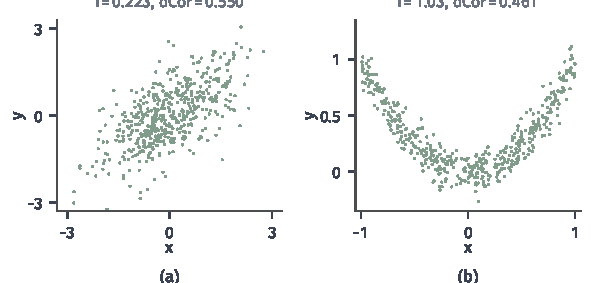
\includegraphics[width=100mm]{figures/07-probability/04-distribution-analysis/matplotlib/dep-ranking/figure.pdf}
  \caption{两个依赖度量给出相反次序的一对分布，各$500$个样本（绿，种子$719$）。(a)$\rho=0.6$的标准二元高斯；(b)$X\sim\operatorname{Unif}(-1,1)$，$Y=X^{2}+0.1Z$。图上方是总体互信息（nat）与距离相关：互信息认为(b)更强，距离相关认为(a)更强。}
  \label{fig:dep-ranking}
\end{BookInlineFigure}

两种判断都有道理，它们回答的是不同的问题。(b)中知道$X$以后，$Y$被限制在抛物线附近宽约$0.1$的窄带里，不确定性大幅减少，所以互信息大。但$X$的一对取值相距远时，$Y$的一对取值未必相距远：$X=\pm0.8$相距$1.6$，对应的$Y$几乎相同。距离相关问的是距离的同步，抛物线的折返削弱了这种同步，所以它更小。HSIC的次序还要看带宽：若两个坐标的带宽都取$1$，表~\ref{tab:dep-values}中高斯更大；若带宽取各坐标的标准差，(b)的HSIC约为$0.0286$，(a)约为$0.0166$，次序又与互信息一致。

\paragraph{真实值与可计算的下界}
互信息还有一个使用上的问题。连续抛物线的互信息是$+\infty$，$\sigma=0.1$的含噪抛物线是$1.03$，而数值方法得到的常常只是一个下界。第~\ref{chap:information-measures}章的InfoNCE下界在$N$个候选时不超过$\ln N$，候选数或评分函数的限制会让下界远低于真实值，并且对不同分布低估的程度不同。比较两个分布的互信息时，要比较的是真实值；拿两个下界的大小作比较，次序可能与真实值相反。

\paragraph{选择依赖度量}
没有一个度量能脱离任务给出统一的强度刻度。若关心的是一个变量能为另一个提供多少信息，且希望结果不受坐标和单位影响，用互信息，并准备好处理无穷大与估计困难。若变量是欧氏空间中的向量，希望用距离和有界的数值描述“取值是否一起变化”，用距离相关，并先统一各坐标的单位。

若变量取值于一般空间（文本、图、函数），或需要在特定尺度上检查依赖，用HSIC，并把核与带宽作为结论的一部分报告。若希望在给定分辨率下读出一张可解释的概率表，用离散化评分，并说明划分方式与归一化规则。几种量能同时判别独立，却可能给出不同的非零排序，选择之前先说清楚要比较的是哪一种依赖。
